%%%%%%%%%%%%%%%%%%%%%%%%%%%%%%%%%%%%%%%%%
% a0poster Landscape Poster
% LaTeX Template
% Version 1.0 (22/06/13)
%
% The a0poster class was created by:
% Gerlinde Kettl and Matthias Weiser (tex@kettl.de)
% 
% This template has been downloaded from:
% http://www.LaTeXTemplates.com
%
% License:
% CC BY-NC-SA 3.0 (http://creativecommons.org/licenses/by-nc-sa/3.0/)
%
%%%%%%%%%%%%%%%%%%%%%%%%%%%%%%%%%%%%%%%%%

%----------------------------------------------------------------------------------------
%	PACKAGES AND OTHER DOCUMENT CONFIGURATIONS
%----------------------------------------------------------------------------------------

\documentclass[a0, landscape]{a0poster}


\usepackage{multicol} % This is so we can have multiple columns of text side-by-side
\columnsep=35pt % This is the amount of white space between the columns in the poster
%\columnseprule=3pt % This is the thickness of the black line between the columns in the poster
%\usepackage{graphicx}
%\usepackage{pstricks,pst-grad}
\usepackage[svgnames]{xcolor} 
\usepackage{booktabs}
\usepackage[absolute]{textpos}
\renewcommand{\familydefault}{\sfdefault}

\usepackage{setspace}
\definecolor{CornellRed}{RGB}{179, 27, 27} % UBC Blue (primary)

\usepackage[left=5cm,right=5cm,bottom=1cm,top=5cm]{geometry}
\usepackage{titlesec}

\usepackage{graphicx} % Required for including images
\usepackage{pstricks,pst-grad}
%\graphicspath{{/Users/shashanksule/Downloads/OrthogonalPolynomials/}} % Location of the graphics files
\usepackage{booktabs} % Top and bottom rules for table
\usepackage[font=small,labelfont=bf]{caption} 
\usepackage{amsfonts, amsmath, amsthm, amssymb} % For math fonts, symbols and environments
\usepackage{wrapfig} % Allows wrapping text around tables and figures


\usepackage{natbib}
\renewcommand{\bibsection}{}
\newcommand{\inner}[2]{\left \langle #1, #2\right \rangle}
\usepackage{tikz}


\usepackage{xcolor}

\begin{document}


\begin{minipage}{\linewidth}
    \begin{center}
    \linespread{1.5}
    \color{CornellRed} \Huge \textbf{Chebyshev and Sobolev Orthogonal Polynomials on the Sierpinski Gasket}
        
                \color{Black}
                \LARGE  Max Jiang, Tian Lan, Shashank Sule, Sreeram Venkat, and Xiaoduo Wang
                
                 % Author(s)
                
                \LARGE  Advisors: Robert Strichartz and Kasso Okoudjou
                
                %\LARGE Cornell SPUR 2019: Analysis on Fractals% University/organization
                
                \end{center}
  \end{minipage}

{%
\begin{textblock*}{10.75in}(4cm,15cm)%
    \begin{minipage}{10.75in} 
    \begin{center}
            {\LARGE \textcolor{CornellRed}{\textbf{Introduction}}}
        \end{center}
        \vspace{1cm}
        We define a Sobolev inner product on the Sierpinski Gasket (SG) and discuss the properties of the corresponding orthogonal polynomials such as recurrence relations, finer estimates, and convergence with respect to parameters in the inner product. Furthermore, we define the Chebyshev polynomials on SG and find the first two Chebyshev polynomials in each monomial family. 
        \vspace{1cm}
        \begin{center}
            {\LARGE \textcolor{CornellRed}{\textbf{Preliminaries}}}
        \end{center}
        \vspace{1cm}
        \begin{itemize}
            \item Let $V_0 = \{q_0, q_1, q_2\} \in \mathbb{R}^2$ and $F_i(x) = \frac{1}{2}(x+q_i)$ for $i=0,1,2$.
            $$SG = \overline{\bigcup_{m=1}^{\infty}\bigcup_{|w|=m}F_w(V_0)}$$
            Here $|w| = m \iff w \in \{0,1,2\}^{m}$ and $F_w = F_{i_m}\circ \cdots \circ F_{i_1}$ where $w = i_m\ldots i_1$
            \item We work on the finite graph approximation $V_m = \bigcup_{|w|=m}F_{w}(V_0)$
            \begin{center}
            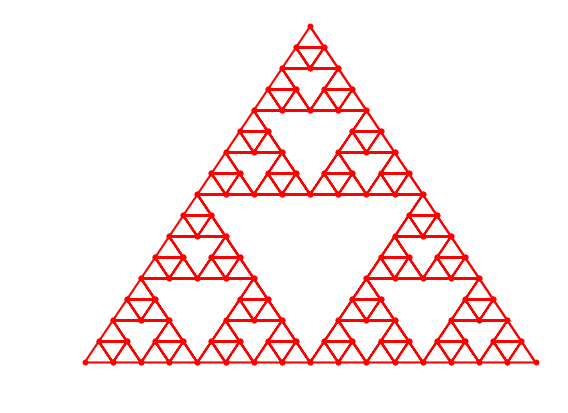
\includegraphics[width=0.45\linewidth]{Final_presentation/images/V4.png}
            \captionof{figure}{\textcolor{CornellRed}{$V_4$}}
            \label{fig:V4}    
            \end{center}
            \item Let $u: SG \mapsto \mathbb{R}$. Then the \textbf{Laplacian} $\Delta_{\mu}$ is 					defined as
        $$  \Delta_{\mu}u(x) = \frac{3}{2}\lim_{m \to \infty}5^m\Delta_mu(x)$$
        \item $G: SG \times SG \mapsto R$ is called \textbf{Green's Function} where
        $$ -\Delta u = f, u|_{V_0} = 0 \iff u(x) = \int_{SG}G(x,y)f(y)\,d\mu$$
            \item The space of polynomials with degree $\le j$ is denoted $\mathcal{H}_{j}$
            \item We use the following basis $\{P_{jk}\}$ for $\mathcal{H}_m$ where $0 \leq j \leq m$ and $k=1,2,3$:
            $$\Delta^nP_{jk}(q_0) = \delta_{nj}\delta_{k1}$$
            $$\Delta^n\partial_nP_{jk}(q_0) = \delta_{nj}\delta_{k2}$$
            $$\Delta^n\partial_TP_{jk}(q_0) = \delta_{nj}\delta_{k3}$$
            This is known as the \textbf{monomial basis}.
            \item Let $f$ and $g$ be polynomials on $SG$. Then the \textbf{Sobolev-$m$ inner product} is defined as follows: 
            
            $$\langle f,g\rangle_{H^m}= \sum\limits_{l = 0}^m \lambda_l\int_{SG}\Delta ^lf\Delta ^lg\,d\mu+\sum\limits_{l=0}^{m-1}\beta_l\,\varepsilon(\Delta ^l f,\Delta ^l g)+\nonumber$$
            $$\sum\limits_{l=0}^{m-1}[\Delta  ^lf(q_0)\,\Delta  ^lf(q_1)\,\Delta  ^lf(q_2)] M_l [\Delta  ^lg(q_0)\,\Delta  ^lg(q_1)\,\Delta  ^lg(q_2)]^T$$
            
            Here $\lambda_l, \beta_l >0$ and $M$ is a $3\times3$ symmetric positive definite matrix. For most of our results we use the $H^1$ inner product where $m=1$ and $M = 0$. 
            \item Fix $k=1,2$ or $3$ and let $M_{nk} = \{f \mid f = \sum_{j=0}^{n}a_jP_{jk}, a_n=1\}$. Then the $\textbf{nth Chebyshev polynomial}$, $T_{nk}$ is defined to be the polynomial $g$ such that 
            $$ g := \min_{f \in M_{nk}}||f||_{\infty}$$
        \end{itemize}
  \end{minipage}%
  \end{textblock*}%
}

{%
\begin{textblock*}{22.5in}(33.31cm,15cm)%
    \begin{minipage}{22.5in}
      \begin{center}
        {\LARGE \textcolor{CornellRed}{\textbf{Experimental Results and Applications}}}
      \end{center}
        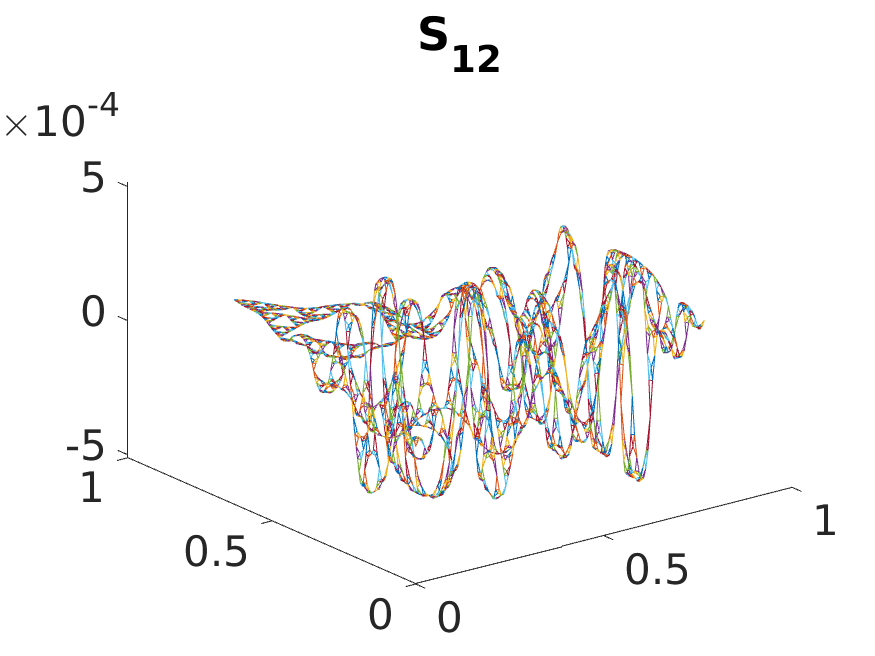
\includegraphics[width=0.33\linewidth]{images/H1AntisymOPs0_23/SAntiSym12.png}
        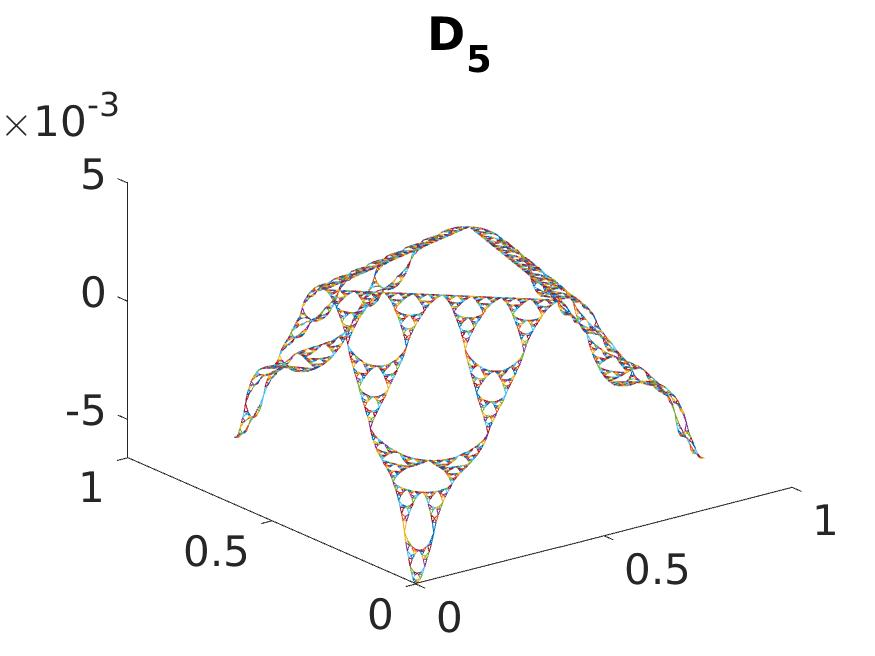
\includegraphics[width=0.33\linewidth]{images/H1SymmOPs0_19/Ss5.jpg}
        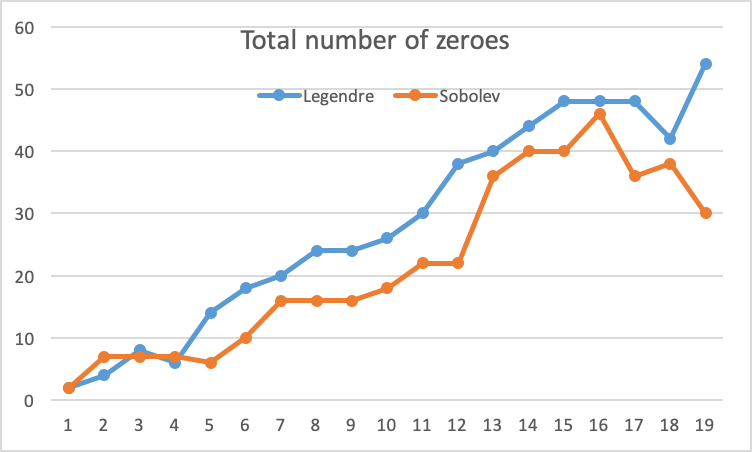
\includegraphics[width=0.33\linewidth]{images/TotalZeroes.png}
        \captionof{figure}{Degree 12 Anti-symmetric Sobolev polynomial, Degree 5 Symmetric Sobolev polynomial, Comparison between zeroes of Legendre and Sobolev polynomials on the edges}
        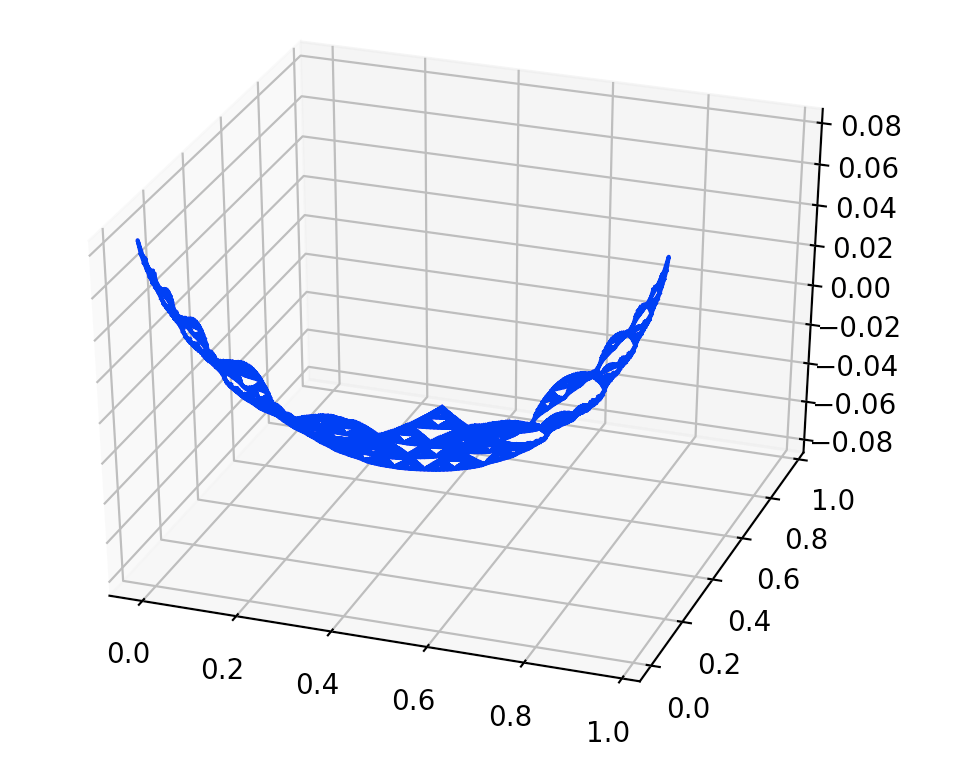
\includegraphics[width=0.33\linewidth]{Final_presentation/images/chebyshev_p11_0_0833.png}
        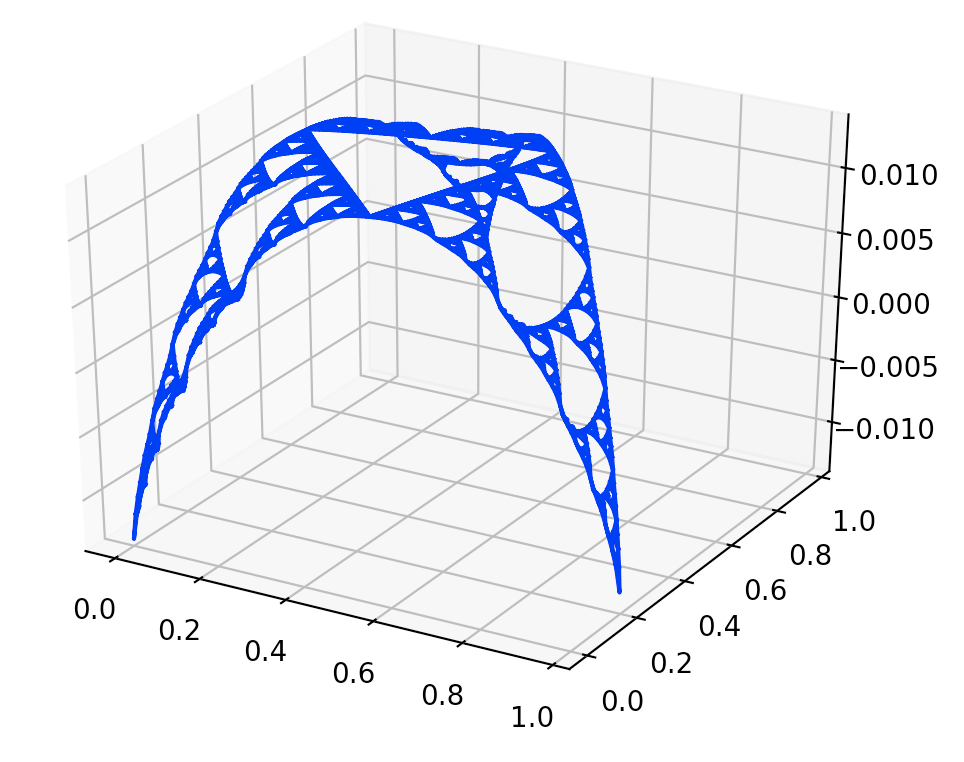
\includegraphics[width=0.33\linewidth]{Final_presentation/images/chebyshev_p12_0_0619339.png}
        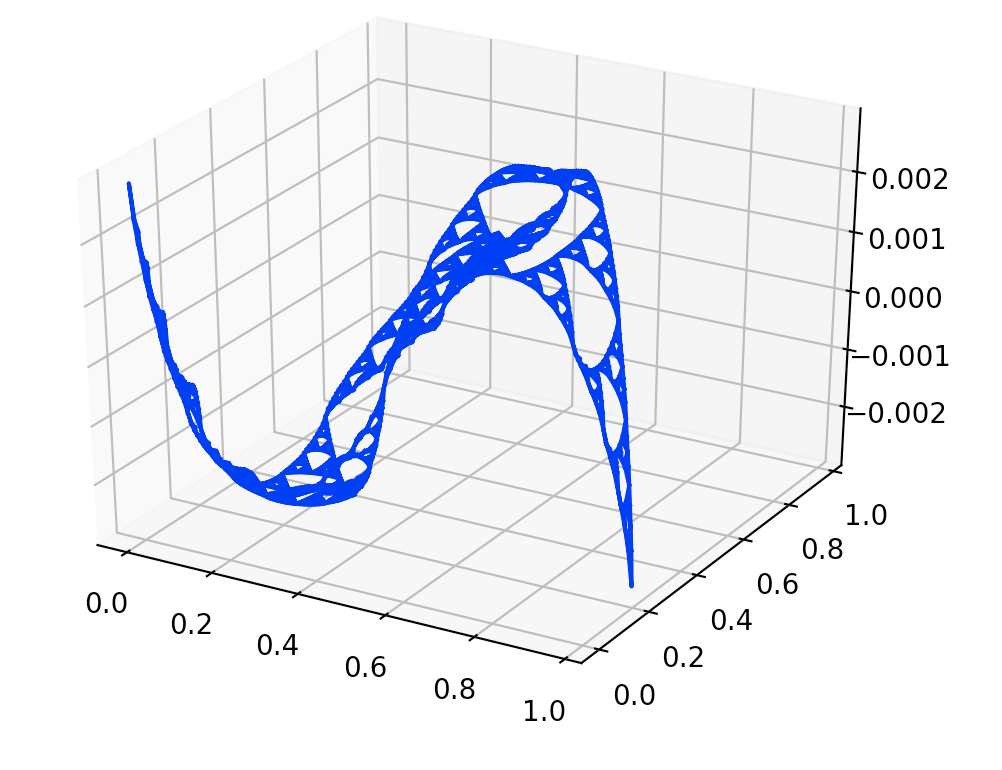
\includegraphics[width=0.33\linewidth]{Final_presentation/images/chebyshev_p13_0_02750235.png}
         \captionof{figure}{Left to right: First Chebyshev polynomials corresponding to $k=1,2,3$}
    \end{minipage}
  \end{textblock*}%
}

{%
\begin{textblock*}{22.5in}(33.31cm,51cm)%
    \begin{minipage}{22.5in}
      \begin{center}
        {\LARGE \textcolor{CornellRed}{\textbf{Theoretical results}}}
      \end{center}
    \begin{multicols}{2}
    \begin{center}
        {\Large \textcolor{CornellRed}{\textbf{Recurrence relations}}}
      \end{center}
    \begin{theorem*}\label{th:gen_rec}
    Suppose $k=2$ or $3$. For the Sobolev-$m$ inner product, we have the following generalized recursion relation for $n\ge -1$
    $$S_{n+m+1} - \mathcal{F}_{n+m+1} - \sum\limits_{l = 0}^{2m-1}a_{n, l}S_{n+m-l} = 0$$
    where
    $$a_{n, l} = -\frac{\inner{\mathcal{F}_{n+m+1}}{S_{n+m-l}}_{H^m}}{\inner{S_{n+m-l}}{S_{n+m-l}}_{H^m}}, \quad \mathcal{F}_{n+m+1} = \mathcal{G}^mp_{n+1}$$
      $$ \mathcal{G}(f)(x) := -\int_{SG}G(x,y)f(y)dy$$
    and $S_j:=0$ if $j<0$.\end{theorem*}
    \begin{theorem*}\label{Recurrence Relation with one assumption $(k=1)$}
    Consider the $H^1$-inner product with $k=1$ and let $\{S_n\}$ and $\{p_n\}$ be the corresonding monic Sobolev orthogonal Legendre polynomials respectively. Additionally, let $S_{-1}:=0$, $f_{n+2}(x) = -\int_{SG}G(x,y)p_{n+1}(y)dy$ and suppose that $\partial_n f_{n+2}(q_0)\neq 0$. Let $n\geq-1$. The Sobolev orthogonal polynomials satisfy the following recurrence relation:
         $$S_{n+3}-a_nS_{n+2} - b_nS_{n+1}-c_nS_n = f_{n+3}+d_nf_{n+2}$$
        The coefficients are given as follows:
        $$ a_n=-\frac{\inner{f_{n+3}+d_nf_{n+2}}{S_{n+2}}_H}{\|S_{n+2}\|_H^2}$$
        $$b_n= -\frac{\inner{f_{n+3}+d_nf_{n+2}}{S_{n+1}}_H}{\|S_{n+1}\|_H^2}$$
        $$ d_n=-\frac{\partial_n f_{n+3}(q_0)}{\partial_nf_{n+2}(q_0)},\:\:c_n=-d_n\frac{\|p_{n+1}\|_{L^2}^2}{\|S_n\|_H^2}\label{d_n and c_n in k=1 recurrence}$$
    \end{theorem*}
    \vfill\null
    \columnbreak
    \begin{center}
        {\Large \textcolor{CornellRed}{\textbf{Convergence properties}}}
    \end{center}
    \begin{theorem*} 
    Suppose $k=2$ or $3$, and there exists $M>0$ such that $\lambda_l\le M$ for any $l<m$. Then there exists positive constants $C_1=C_1(n,\mu)$, $C_2=C_2(n,\mu,M,m)$ such that for any $n\ge 0$, $$C_2 \ge\sum\limits_{l = 0}^{m-1} \lambda_l\int_{SG}(\Delta ^l S_n)^2\,d\mu\ge C_1$$ $$
      C_2+\lambda_m\|p_{n-m}\|_{L^2}^2\ge \|S_n\|_{H^m}^2\ge C_1+
      \lambda_m \|p_{n-m}\|_{L^2}^2$$
      Consequently, for any $n\ge 2m+1$, we have$$\|S_n-\mathcal{F}_n\|_{L^2}\le
      C(n,M,m,\mu)\lambda_m^{-1}$$and
      $\lim\limits_{\lambda_m\rightarrow\infty}\|\Delta^i S_n-\mathcal{G}^{m-i}p_{n-m}\|_{L^\infty}\rightarrow 0$ for any $0\le i\le m$.
    \end{theorem*}
    \begin{theorem*}
   Suppose the normal derivative conjecture is true and $k=1$. Then there exists a sequence of monic polynomials $\{g_n\}_{n=0}^{\infty}$ independent of $\lambda$ such that for any $n\ge0$, $deg\, g_n=n$, $S_n$ converges uniformly in $x$ to $g_n$. And $g_{n+3}+d_ng_{n+2}=f_{n+3}+d_nf_{n+2}$ for any $n\ge 1$. For the basic cases, $g_0=p_0$, $g_1=p_1$, $g_{2}+d_{-1}g_{1}=f_{2}+d_{-1}f_{1}-\frac{\langle f_2+d_{-1}f_1,{g_0}\rangle_{L^2}}{{\|g_0\|_{L^2}^2}}g_{0}$, and 
$g_{3}+d_{0}g_{2}=f_{3}+d_{0}f_{2}-\frac{\langle f_3+d_{0}f_2,{g_0}\rangle_{L^2}}{{\|g_0\|_{L^2}^2}}g_{0}$. Moreover, for any $\alpha<1$, $n\ge0$, $\lim\limits_{\lambda \rightarrow\infty}\lambda^\alpha(S_n(\lambda)-g_n)=0$ uniformly in $x$.
    \end{theorem*} 
    \end{multicols}
    \end{minipage}
  \end{textblock*}%
}

{%
\begin{textblock*}{10.75in}(91.46cm,15cm)%
    \begin{minipage}{10.75in} 
    \begin{center}
            {\LARGE \textcolor{CornellRed}{\textbf{Further Research}}}
        \end{center}
        \vspace{1cm}
        \begin{enumerate}
        \item \textbf{Interpolation and Quadrature}: For which points $x_1, \ldots x_{3n+3}$ is the matrix $M_n$ where
        
	$$ M_n = \begin{bmatrix}
    P_{0,1}(x_1) & \ldots & P_{n,3}(x_1) \\
    \vdots & \ddots & \vdots \\
    P_{0,1}(x_{3n+3}) & \ldots & P_{n,3}(x_{3n+3})\\
    \end{bmatrix}$$
        
        invertible? We call $M_n$ the \textbf{interpolation matrix} and the above problem arises when we attempt to interpolate an $n$ degree polynomial with $3n + 3$ distinct points. We have the following lemma: 
\begin{lemma*}
For any $n\ge 0$, take $x_i=F_0^{(i-1)}(q_1)$ for $1\le i\le 2n+2$, and $x_i=F_0^{(i-2n-3)}(q_2)$ for $2n+3\le i \le 3n+3$. Then the matrix \eqref{interpolationmatrix} is invertible.
\end{lemma*}
        
On the other hand, $S_{14}$ has at least 22 zeroes on the left half of $SG$ so if we picked $x_1, \ldots, x_{15}$ to be any 15 of these points then $M_{14}$ would not be invertible. Thus the next question is to characterise those sets for which $M_n$ is invertible. But due to the above lemma we have a quadrature rule $I^{m}_{n}$ that integrates $n$-harmonic splines exactly. We have the following estimate for the error: 
        
     $$ \left|I_n^m(f) - \int_{SG}f\right|\leq c_1(n)5^{-(n+1)m}\|\Delta^{(n+1)}f\|_\infty$$
        \item \textbf{Normal derivative conjecture}: Let $f_t = -\int_{SG}G(x,y)p_{t-1}\,dx$ where $p_{t-1}$ is the $t-1$th Legendre polynomial from the $k=1$ family. Is $\partial_{n}f_{t}(q_0) \neq 0$? Values of $\partial_{n}f_{t}(q_0) \neq 0$ have been verified up to $t=120$. We require this conjecture for the recurrence relation in the $k=1$ case. 
       \item \textbf{Computing higher degree Chebyshev polynomials}: For the $2^{nd}$ Chebyshev polynomials of the families $k=2$ and$ 3$, we can numerically find that $a_{2} = −0.0619339$ and $a_{3} = −0.0275013$. However, the general form of Chebyshev polynomials and their properties such as orthogonality, recursion, and alternation are still unexplored. \nocite{*}
\end{enumerate}         
        \vspace{1cm}
        \begin{center}
            {\LARGE \textcolor{CornellRed}{\textbf{References}}}
        \end{center}
        \vspace{1cm}
        \bibliographystyle{plain}
        \bibliography{ReferencesForPaper}
        %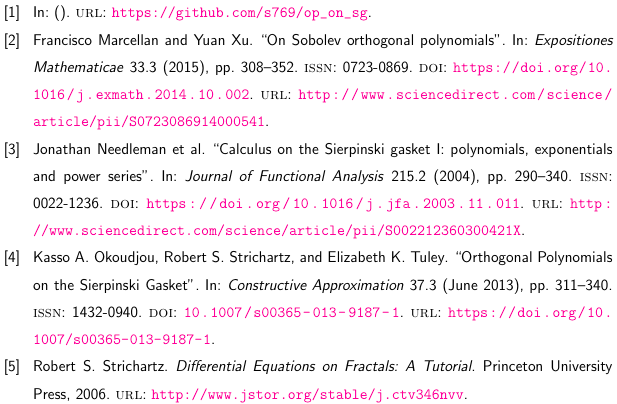
\includegraphics[width=\linewidth]{Poster/Referencex.png}
      \vspace{1cm}
        %\begin{center}
          %  {\LARGE \textcolor{CornellRed}{\textbf{Acknowledgements}}}
        %\end{center}
        %\vspace{1cm}
        We thank our advisors, Kasso Okoudjou and Robert Strichartz for introducing us to Analysis on Fractals and for their encouragement throughout. We also express our gratitude towards the Cornell SPUR 2019 and PIRIP programs at Cornell University for supporting our work. 
  \end{minipage}%
  \end{textblock*}%
}


   

\end{document}